\documentclass[journal,10pt,twocolumn]{article}
\usepackage[margin=0.5in]{geometry}
\usepackage[cmex10]{amsmath}
\usepackage{array}
\usepackage{booktabs}
% The preceding line is only needed to identify funding in the first footnote. If that is unneeded, please comment it out.
\usepackage{cite}
\usepackage{amsmath,amssymb,amsfonts}
\usepackage{graphicx}
\usepackage{textcomp}
\usepackage{xcolor}
\usepackage{graphicx}
\graphicspath{{./fig}}{}
\def\BibTeX{{\rm B\kern-.05em{\sc i\kern-.025em b}\kern-.08em
    T\kern-.1667em\lower.7ex\hbox{E}\kern-.125emX}}
\usepackage{tikz}
\usetikzlibrary{shapes.geometric}
\usetikzlibrary{shapes.geometric,angles,quotes}
\begin{document}
\newtheorem{theorem}{Theorem}[section]
\newtheorem{problem}{Problem}
\newtheorem{proposition}{Proposition}[section]
\newtheorem{lemma}{Lemma}[section]
\newtheorem{corollary}[theorem]{Corollary}
\newtheorem{example}{Example}[section]
\newtheorem{definition}[problem]{Definition}
%\newtheorem{thm}{Theorem}[section] 
%\newtheorem{defn}[thm]{Definition}
%\newtheorem{algorithm}{Algorithm}[section]
%\newtheorem{cor}{Corollary}
\newcommand{\BEQA}{\begin{eqnarray}}
\newcommand{\EEQA}{\end{eqnarray}}
\newcommand{\define}{\stackrel{\triangle}{=}}
\newcommand*\circled[1]{\tikz[baseline=(char.base)]{
    \node[shape=circle,draw,inner sep=2pt] (char) {#1};}}
\bibliographystyle{article}
%\bibliographystyle{ieeetr}
\providecommand{\mbf}{\mathbf}
\providecommand{\pr}[1]{\ensuremath{\Pr\left(#1\right)}}
\providecommand{\re}[1]{\ensuremath{\text{Re}\left(#1\right)}}
\providecommand{\im}[1]{\ensuremath{\text{Im}\left(#1\right)}}
\providecommand{\qfunc}[1]{\ensuremath{Q\left(#1\right)}}
\providecommand{\sbrak}[1]{\ensuremath{{}\left[#1\right]}}
\providecommand{\lsbrak}[1]{\ensuremath{{}\left[#1\right.}}
\providecommand{\rsbrak}[1]{\ensuremath{{}\left.#1\right]}}
\providecommand{\brak}[1]{\ensuremath{\left(#1\right)}}
\providecommand{\lbrak}[1]{\ensuremath{\left(#1\right.}}
\providecommand{\rbrak}[1]{\ensuremath{\left.#1\right)}}
\providecommand{\cbrak}[1]{\ensuremath{\left\{#1\right\}}}
\providecommand{\lcbrak}[1]{\ensuremath{\left\{#1\right.}}
\providecommand{\rcbrak}[1]{\ensuremath{\left.#1\right\}}}
\newcommand{\sgn}{\mathop{\mathrm{sgn}}}
%\providecommand{\hilbert}{\overset{\mathcal{H}}{ \rightleftharpoons}}
\providecommand{\system}{\overset{\mathcal{H}}{ \longleftrightarrow}}
	%\newcommand{\solution}[2]{\textbf{Solution:}{#1}}
\newcommand{\solution}{\noindent \textbf{Solution: }}
\newcommand{\cosec}{\,\text{cosec}\,}
\providecommand{\dec}[2]{\ensuremath{\overset{#1}{\underset{#2}{\gtrless}}}}
\newcommand{\myvec}[1]{\ensuremath{\begin{pmatrix}#1\end{pmatrix}}}
\newcommand{\mydet}[1]{\ensuremath{\begin{vmatrix}#1\end{vmatrix}}}
	\newcommand*{\permcomb}[4][0mu]{{{}^{#3}\mkern#1#2_{#4}}}
\newcommand*{\perm}[1][-3mu]{\permcomb[#1]{P}}
\newcommand*{\comb}[1][-1mu]{\permcomb[#1]{C}}
%\numberwithin{equation}{section}
\numberwithin{equation}{subsection}
%\numberwithin{problem}{section}
%\numberwithin{definition}{section}
\let\vec\mathbf
\title{
{Deriving the equation of Circle with given parameters \\
Using Matrices}\\
}
\author{Bavya}
\maketitle
\tableofcontents
\section{Problem statement}
Intercept on the line y=x by the circle $x^2+y^2-2x=0$ is AB. Equation of the circle on AB as a diameter is.
\section{Considerations}
\vspace{0.2cm}
The input parameters are the lengths r, c and angle $\theta$. \\
\vspace{0.2cm}
{
\setlength\extrarowheight{2pt}
\begin{tabular}{|c|c|}
	\hline
	\textbf{Symbol}&\textbf{Description}\\
	\hline
	$x^2+y^2-2x=0$ 
	&Given circle\\
	\hline
	y=x&Diameter of the required Circle\\
	\hline
	$\vec{C}=\myvec{x \\ y}$ &Center of the required Circle
	\\
\hline
\end{tabular}
}
\section{Plotting the Circle with center and radius}
\vspace{0.25cm}
Plot of the Circle with center $\vec{C} =\myvec{\frac{1}{2} \\ \frac{1}{2}}$ and radius r=0.707  is shown in figure 1, .
\begin{figure}[h]
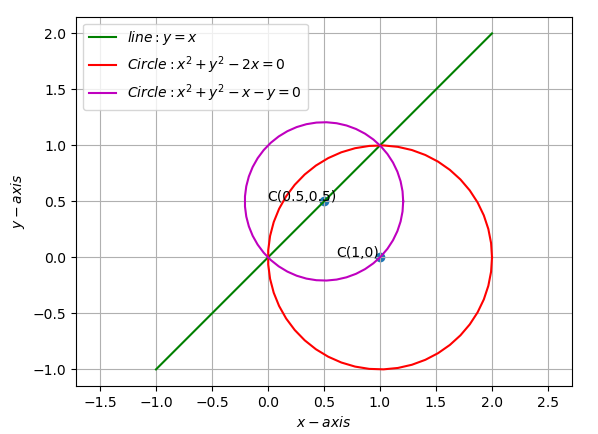
\includegraphics[width=1\columnwidth]{circle.png}
\caption{Circle with radius r=0.707 and center C($\frac{1}{2}, \frac{1}{2})$}
\label{fig:Circle with radius and center}
\end{figure}
\section{Solution}
\vspace{0.25cm}

\begin{flushleft}

As per given data, equations of diameter line and circle  are
\begin{equation}
y=x 
\end{equation}
\begin{equation}
x^2+y^2-2x=0
\end{equation}
The above equations can be written in matrix form as,
\begin{equation}
    \myvec{ 1\\-1} \vec{x} = 0
\end{equation}
\begin{equation}
   \vec{x}^T \vec{V} \vec{x} + 2 \myvec{-1 & 0} \vec{x}=0
\end{equation}

\begin{flushleft}
On solving above equations, we get two end points of diameter,
\end{flushleft}
\begin{equation}
    \vec{A}=\myvec{ 0 \\ 0} , \vec{B}=\myvec{1 \\ 1} 
\end{equation}
\subsection{Calculation of center of the Circle}
\begin{flushleft}
From Point A and B, we can find the center of the required circle as,\\
\end{flushleft}
\begin{equation}
\vec{C}=\frac{\vec{A+B}}{2} = \myvec{\frac{1}{2}\\\frac{1}{2}}    
\end{equation}
\end{flushleft}

\subsection{Calculation of radius of the Circle}
As per the given data, y=x is the diameter of the required circle and it is also calculated that the Points A and B are end points of the diameter,\\
Let r be the radius of circle,\\
\begin{equation}
r= \frac{\vec{||A-B||}}{2} = \frac{\sqrt{2}}{2}=0.707
\end{equation}

\subsection{Deriving equation for Circle in matrix form}
\vspace{0.2cm}
\begin{flushleft}
The equation of circle in matrix form is,\\
\vspace{0.25cm}
\end{flushleft}
\vspace{0.25cm}
\begin{equation}
 \vec{x}^T \vec{V} \vec{x} + 2 \vec{u}^T \vec{x} + f = 0
\end{equation}
\endcenter

\begin{flushleft}
where,\\
\end{flushleft}
\center
$\vec{V} = \vec{I}= \myvec{ 1 & 0\\ 0 & 1}, \vec{u} = \myvec{-\frac{1}{2} \\ -\frac{1}{2}}, f = ||\vec{u}||^2 - r^2 =\frac{1}{2}-\frac{1}{2}=0$\\
\endcenter
\begin{equation}
\implies \vec{x}^T\vec{I}\vec{x}  + 2  \myvec{-\frac{1}{2}&-\frac{1}{2}} \vec{x} = 0
\end{equation}
\begin{equation}
   \implies  \vec{x}^T\myvec{1&0\\0&1} \vec{x}  + 2  \myvec{-\frac{1}{2}&-\frac{1}{2}} \vec{x}= 0 
\end{equation}
 \begin{flushleft}
\vspace{0.23cm}
Therefore, the circle equation can be written as
\end{flushleft}
\begin{equation}
    \vec{x}^T \vec{x} + 2 \myvec{-\frac{1}{2}&-\frac{1}{2}} \vec{x}= 0
\end{equation}
\endcenter


\section{Conclusion}
\begin{flushleft}
1. At first, end points of diameter ($\vec{A}\ and\ \vec{B}$) have been found from the given data.\\
\vspace{0.25cm}
2. Radius of the center has been calculated from $\vec{A}\ and\ \vec{B}$.\\
\vspace{0.25cm}
3. Matrix equation for $\vec{V, u, u^T}$ and $f$ has been derived.\\
\vspace{0.25cm}
4. Finally, the Circle equation has been derived as, \\
\end{flushleft}

\begin{center}
    $\vec{x}^T \vec{x} + 2 \myvec{-\frac{1}{2}&-\frac{1}{2}} \vec{x}= 0$
\end{center}

\end{document}